\section{Chat}

Chat to bardzo ważna funkcjonalność, która zapewnia istnienie podstawowego kanału komunikacyjnego pomiędzy klientem i wykonawcą. Ekran chatu, z uwzględnieniem obu aplikacji, przedstawiono na rysunku \ref{fig:chat}. Składa się on z kilku części: paska aplikacji, paska statusu oferty, panelu odebranych wiadomości oraz wysyłania nowych.

Na pasku aplikacji umieszczona jest ikona umożliwiająca połączenie telefoniczne z drugą stroną. Jest ono jednak dostępne jedynie wtedy, kiedy uzupełniła ona swój numer telefonu. Jest on bowiem zarówno dla klientów, jak i wykonawców opcjonalny. Na tym pasku jest również umieszczona ikona umożliwiająca rozwinięcie innych opcji. Znajdują się tam elementy zależne od aplikacji. Klienci mają możliwość zobaczenia profilu wykonawcy oraz dodania lub zobaczenia oceny. Wykonawcy mogą natomiast zobaczyć szczegóły zlecenia, przenieść je do archiwalnych lub w drugą stronę oraz zobaczyć ocenę, jeśli jest dodana.

Pasek statusu oferty informuje o aktualnym statusie oraz umożliwia jego zmianę. Po wybraniu innego niż aktualny wyświetlone zostanie okno dialogowe z prośbą o potwierdzenie. Po wykonaniu tej czynności jej status się zmienia, a na chacie zostaje wysłana wiadomość o tym mówiąca.

\begin{figure}[ht]
  \captionsetup[subfigure]{justification=centering}
  \centering
  \begin{subfigure}[t]{0.32\textwidth}
    \centering
    \fbox{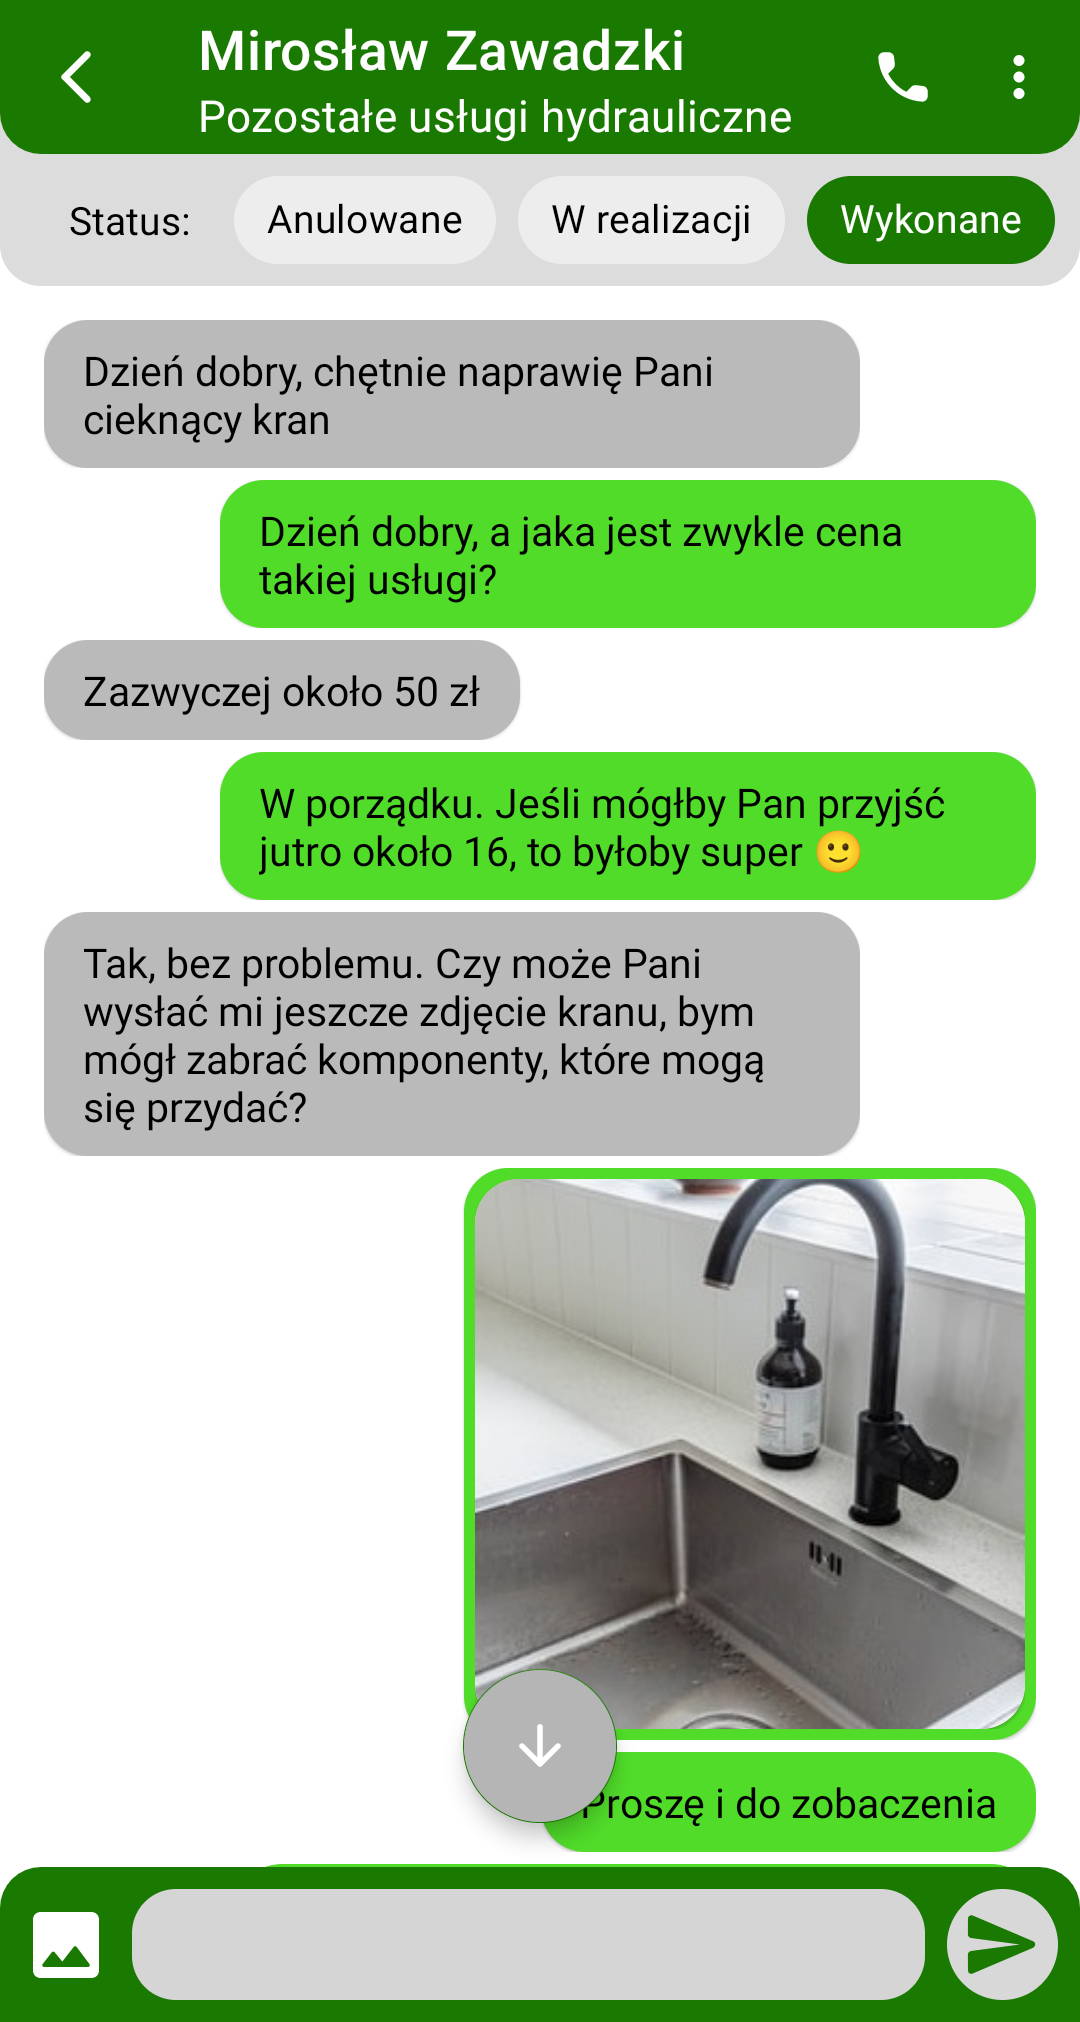
\includegraphics[width=0.97\linewidth]{screens/chat_client.png}}
    \caption{Widok aplikacji dla klientów}
  \end{subfigure}
  \begin{subfigure}[t]{0.32\textwidth}
    \centering
    \fbox{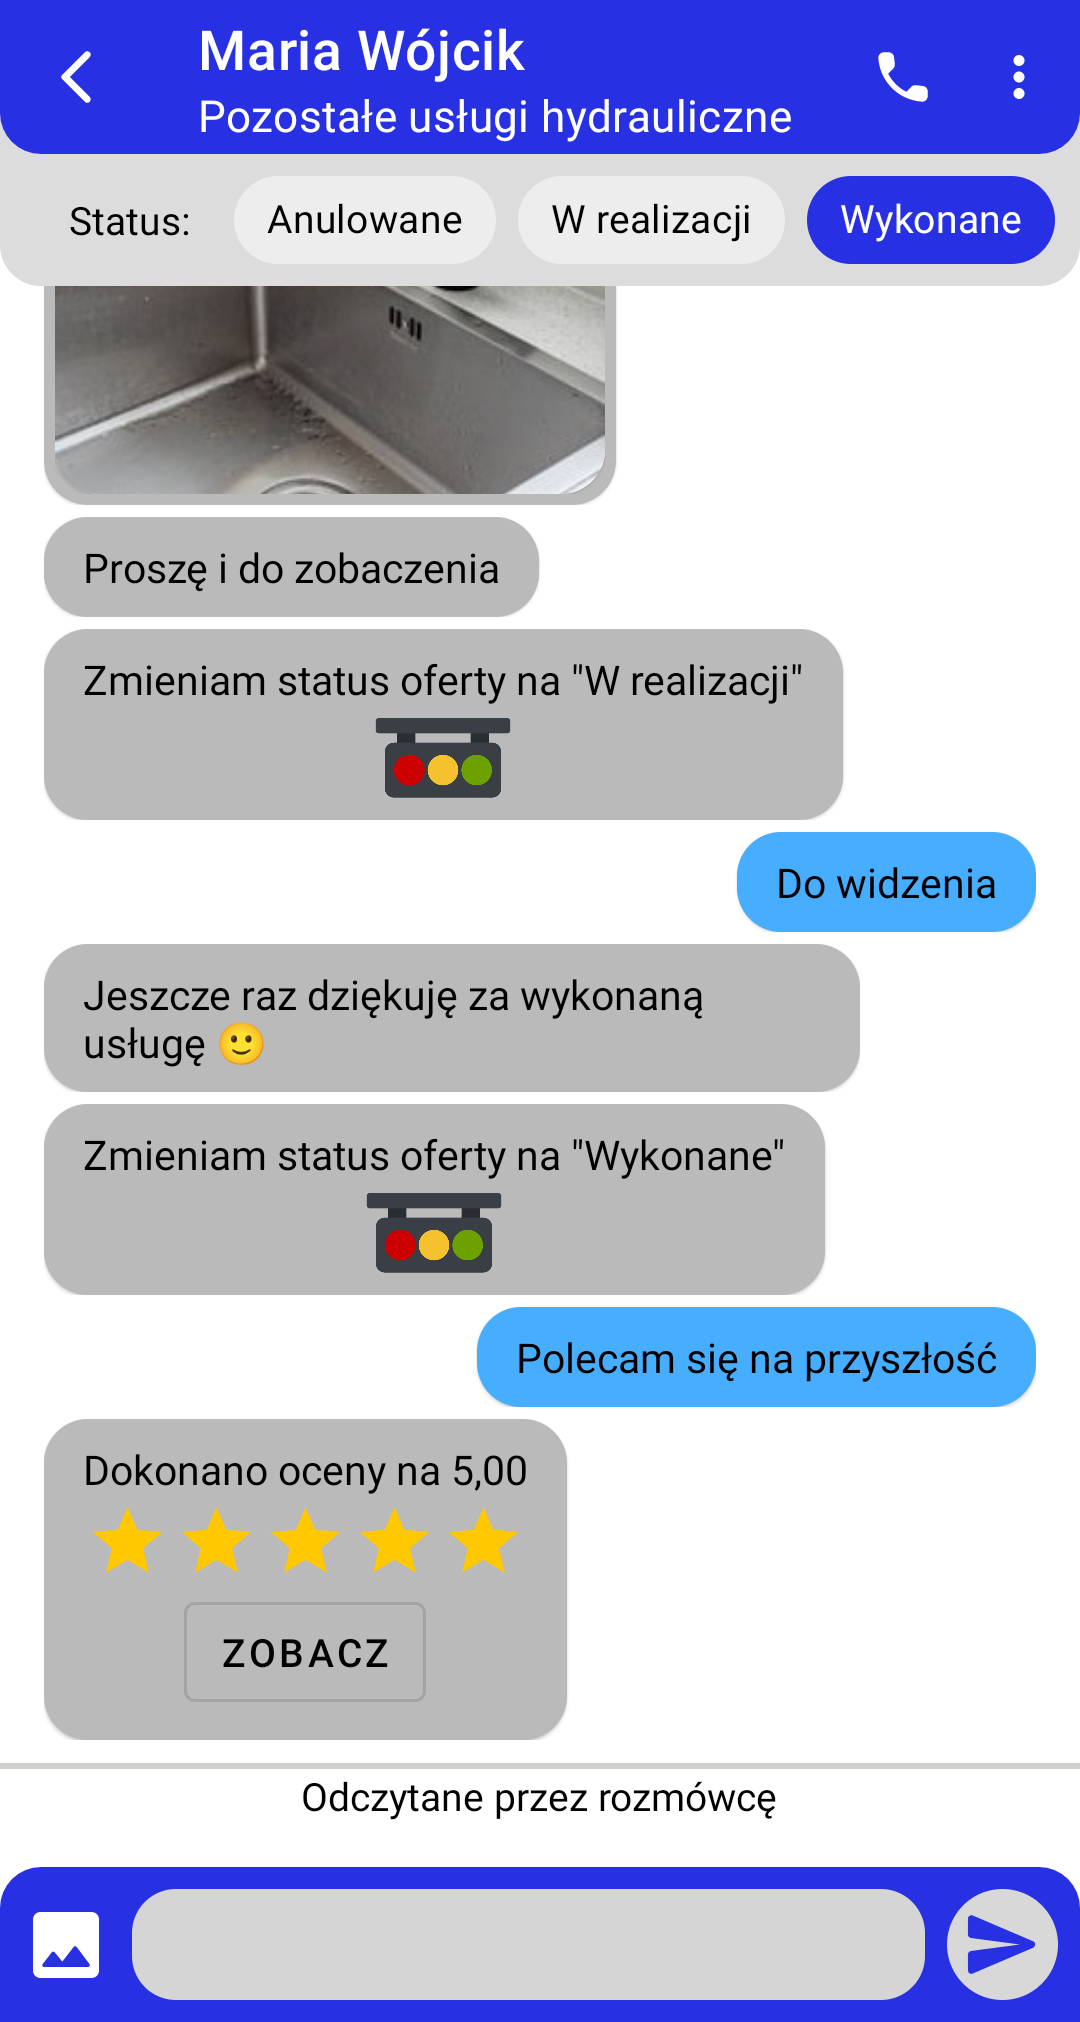
\includegraphics[width=0.97\linewidth]{screens/chat_expert.png}}
    \caption{Widok aplikacji dla wykonawców}
  \end{subfigure}
  \caption{Ekran chatu}
  \label{fig:chat}
\end{figure}

Panel wiadomości zawiera po prawej stronie wiadomości wysyłane, a po lewej odbierane. Występują ich cztery rodzaje: tekstowe, zdjęcia, informujące o zmianach statusu oraz dodaniu komentarza. Są przechowywane w bazie danych we wspólnej kolekcji, lecz dokumenty je reprezentujące posiadają różny zestaw pól, w zależności od wspomnianego typu wiadomości.
Gdy konwersacja zostanie przesunięta do góry, to na dole pojawia się ikona strzałki, która umożliwia szybki powrót do wiadomości najnowszych. Wśród wiadomości widoczna jest również pozioma linia, która jasno oddziela wiadomości odczytane przez rozmówcę od tych nieodczytanych.

Ostatnim elementem jest panel wysyłania wiadomości. Umożliwia on przesyłanie zdjęć oraz komunikatów tekstowych. Dla tych ostatnich operacja jest możliwa do wykonania offline. Obok takich wiadomości wyświetli się informacja o aktualnym braku możliwości wysłania i zostanie to dokonane zaraz po przywróceniu połączenia z siecią. Jest to możliwe dzięki wbudowanemu w bazę Firebase Firestore mechanizmowi pracy offline. Magazyn plików Firebase Storage podobnej funkcjonalności nie posiada i w przypadku braku internetu wysyłanie zdjęcia zwyczajnie się nie powiedzie. Zostanie za to wyświetlony przyjazny komunikat z możliwością ponowienia operacji.